\section{Multiple View Geometry}

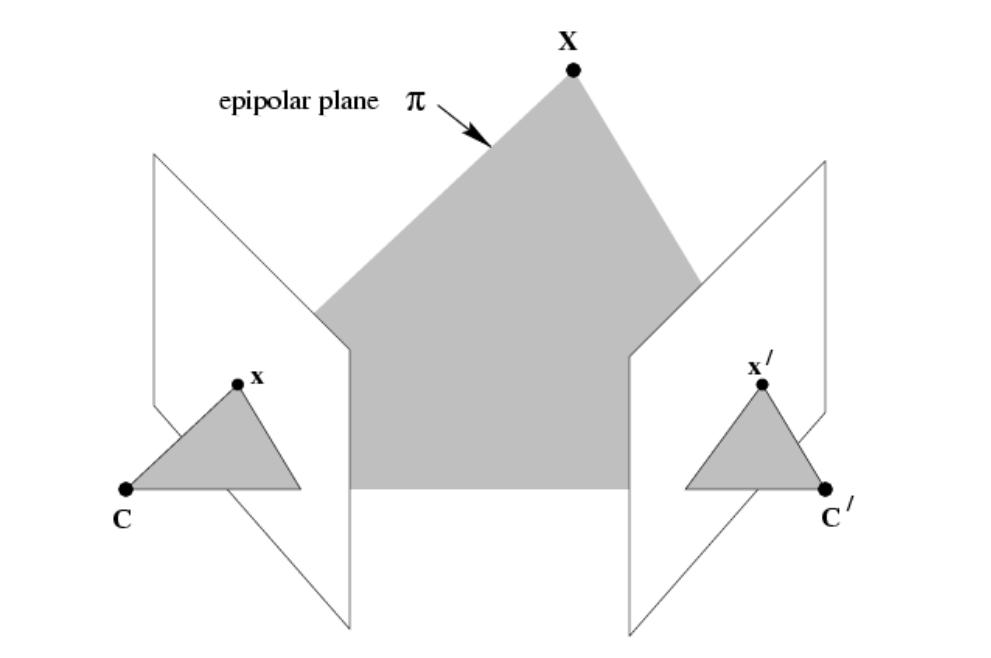
\includegraphics[width=\columnwidth]{pictures/epipolarplane}

All points on $\pi$ project on l and l’

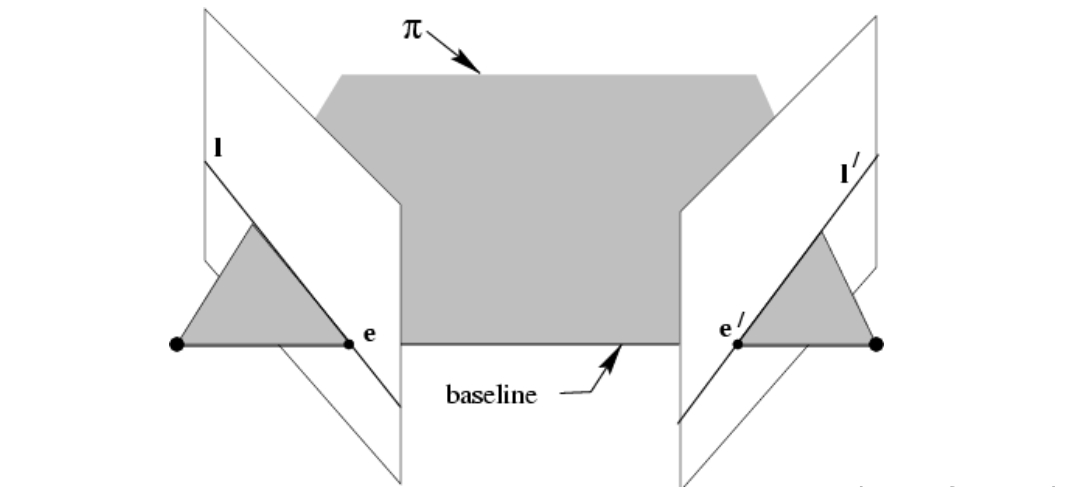
\includegraphics[width=\columnwidth]{pictures/epipolarplane2}

epipoles e,e’
\begin{itemize}
	\item intersection of baseline with image plane
	\item projection of projection center in other image
	\item vanishing point of camera motion direction\\
	\end{itemize}

an epipolar plane ($\pi$)
\begin{itemize}
	\item plane containing baseline (1-D family)\\
\end{itemize}

an epipolar line ($l$) 
\begin{itemize}
	\item intersection of epipolar plane with image (always come in corresponding pairs)\\
\end{itemize}

epipolar lines from motion

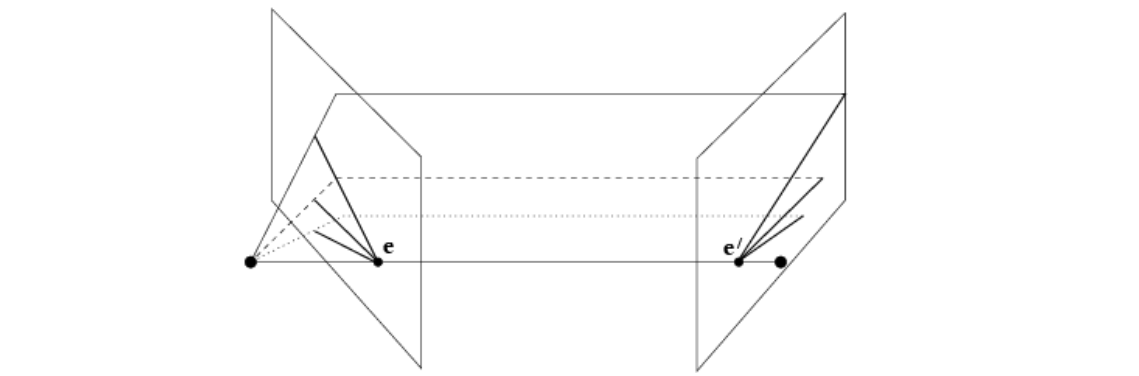
\includegraphics[width=0.8\columnwidth]{pictures/motion}

parallel motion

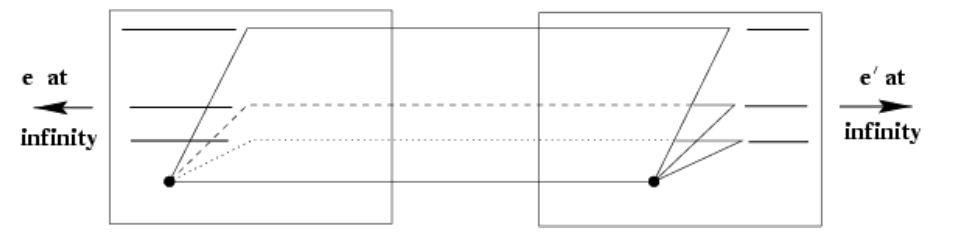
\includegraphics[width=0.8\columnwidth]{pictures/parallelmotion}

forward motion

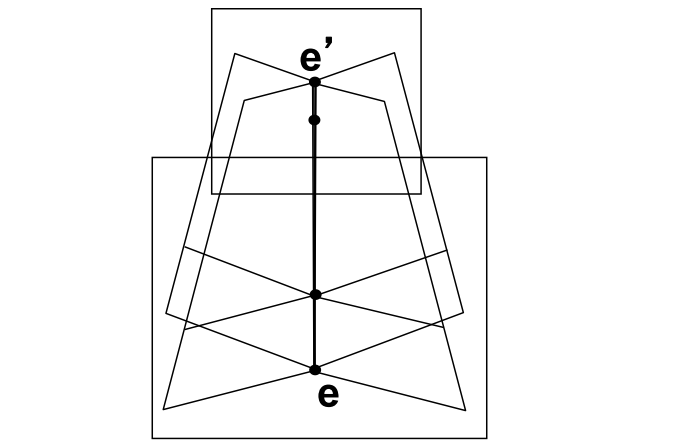
\includegraphics[width=0.4\columnwidth]{pictures/forwardmotion}

\subsection{Fundamental matrix}

$$l' = e' \times x' = e' \times Hx = Fx$$

The fundamental matrix F is independent of the point.

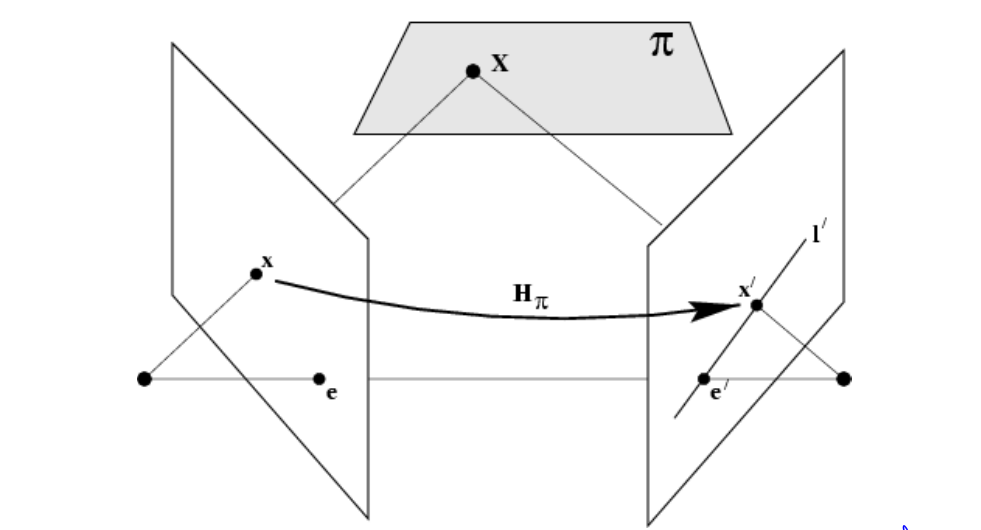
\includegraphics[width=\columnwidth]{pictures/epipolarplane3}

correspondence condition: 
$$x'^TFx=x'^T l'=0$$

\begin{itemize}
	\item transpose: if F is fundamental matrix for (P,P'), then transp(F) is fundamental matrix for (P',P)
	\item Epipolar lines: l'=Fx and l=transp(F)x'
	\item Epipoles: on all epipolar lines, thus transp(e')Fx=0 for all x therefore transp(e')F = 0, similarly Fe=0
	\item F has 7 DOF i.e. 3x3-1(homogeneous)-1(rank2)
	\item F is a correlation, projective mapping from a point x to a line l'=Fx (not a proper correlation, i.e. not invertible)
\end{itemize}

for pure translation F only has 2 degrees of freedom

\subsubsection{Eight-Point Algorithm}
Since the fundamental matrix F is a 3x3 matrix determined up to an arbitrary scale factor, 8 linear equations are required to obtain a unique solution. It is possible with 7.

\subsection{Essential Matrix}
for the calibrated case

5 linear equations are needed.

Same as Fundamental matrix
\begin{itemize}
	\item Ep' is the epipolar line associated with p'
	\item transp(E)p is the epipolar line associated with p
	\item Ee'=0 and transp(E)e=0
	\item E is singular
\end{itemize}

New

\begin{itemize}
	\item E has two equal non-zero singular values
\end{itemize}


\subsection{Multi-view geometry}


\subsection{Dealing with Wide FOV Camera}
\begin{itemize}
	\item Two-step linear approach to compute radial distortion
	\item estimates distortion polynomial of arbitrary degree
\end{itemize}